\documentclass[border=10pt]{standalone}
\usepackage[svgnames]{xcolor}
\usepackage{amsmath}
\usepackage{pgfplots}
\pgfplotsset{compat=newest}
\usepackage[sfdefault]{FiraSans}
\usepackage{FiraMono}
\renewcommand*\familydefault{\sfdefault}
\begin{document}
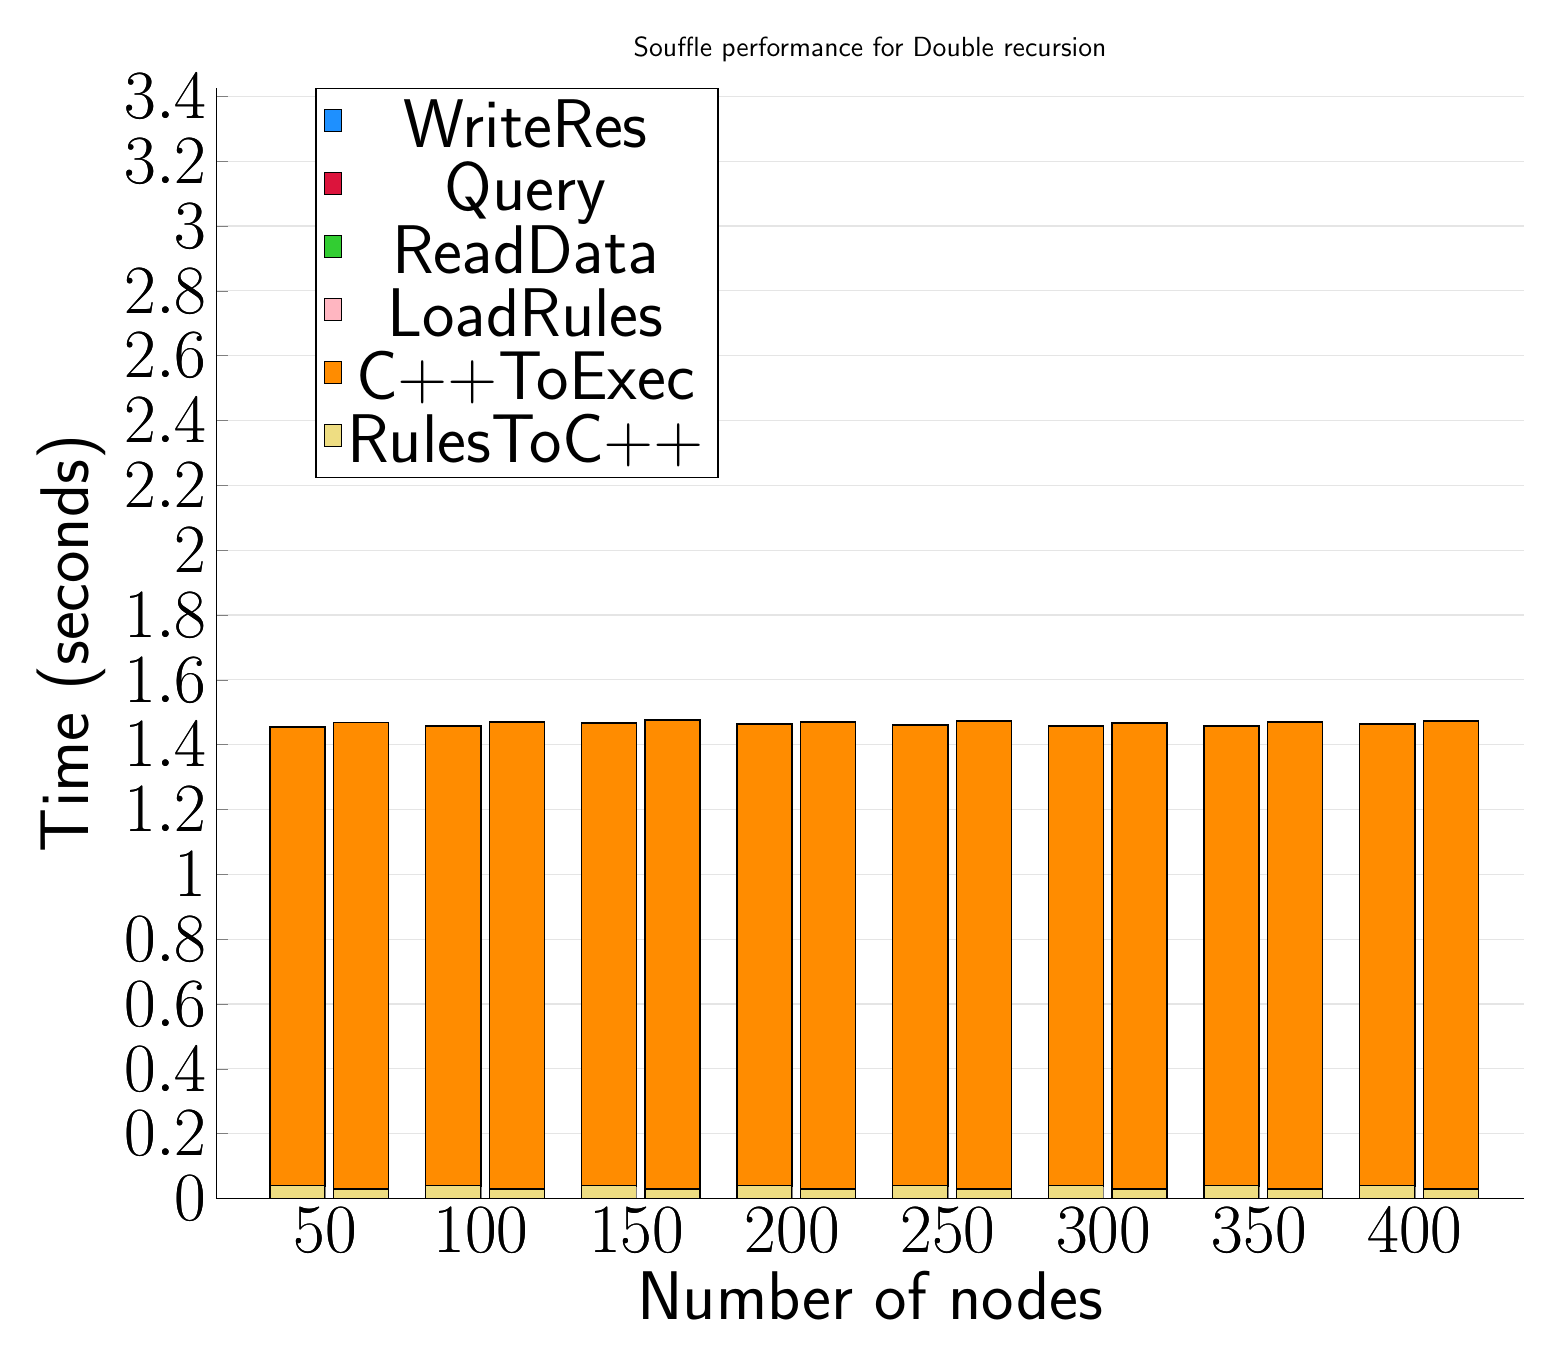
\begin{tikzpicture}
\begin{axis}[
   ybar stacked,
   title={Souffle performance for Double recursion},
   bar shift=-10pt,
   width=1.5\textwidth,
   bar width=0.7cm,
   ymajorgrids, tick align=inside,
   major grid style={draw=gray!20},
   xtick=data,
   ymin=0, ymax=3.4260000705718996,
   axis x line*=bottom,
   axis y line*=left,
   enlarge x limits=0.1,
   legend style={
       at={(0.23, 1)},
       anchor=north,
       legend columns=1,
       font=\Huge,
   },
   ylabel={Time (seconds)},
   xlabel={Number of nodes},
   label style={font=\Huge},
   tick label style={font=\Huge},
]
\addlegendimage{fill=DodgerBlue, draw=black, line width=0.2pt}
\addlegendentry{WriteRes}
\addlegendimage{fill=Crimson, draw=black, line width=0.2pt}
\addlegendentry{Query}
\addlegendimage{fill=LimeGreen, draw=black, line width=0.2pt}
\addlegendentry{ReadData}
\addlegendimage{fill=LightPink, draw=black, line width=0.2pt}
\addlegendentry{LoadRules}
\addlegendimage{fill=DarkOrange, draw=black, line width=0.2pt}
\addlegendentry{C++ToExec}
\addlegendimage{fill=LightGoldenrod, draw=black, line width=0.2pt}
\addlegendentry{RulesToC++}
\addplot +[fill=LightGoldenrod, draw=black, line width=0.5pt] coordinates {
    (50, 0.04000003337860107)
    (100, 0.04000000953674317)
    (150, 0.039999961853027344)
    (200, 0.04000005722045898)
    (250, 0.039999985694885255)
    (300, 0.039999985694885255)
    (350, 0.039999985694885255)
    (400, 0.039999985694885255)
};
\addplot +[fill=DarkOrange, draw=black, line width=0.5pt] coordinates {
    (50, 1.4140000104904176)
    (100, 1.4170000076293945)
    (150, 1.4260000705718994)
    (200, 1.421999955177307)
    (250, 1.419000005722046)
    (300, 1.4160000085830688)
    (350, 1.4180000066757201)
    (400, 1.422000026702881)
};
\addplot +[fill=LightPink, draw=black, line width=0.5pt] coordinates {
    (50, 0.00010267510000000002)
    (100, 9.611259999999999e-05)
    (150, 0.0001235751)
    (200, 0.00012569159999999997)
    (250, 0.00012025390000000001)
    (300, 0.00010987489999999998)
    (350, 0.0001251918)
    (400, 0.0001274084)
};
\addplot +[fill=LimeGreen, draw=black, line width=0.5pt] coordinates {
    (50, 0.00033379169999999997)
    (100, 0.00043492929999999996)
    (150, 0.0005711873999999999)
    (200, 0.0006661208)
    (250, 0.0007467459)
    (300, 0.0008524293)
    (350, 0.0009831129)
    (400, 0.001128684)
};
\addplot +[fill=Crimson, draw=black, line width=0.5pt] coordinates {
    (50, 0.0)
    (100, 0.00012866239999999998)
    (150, 0.00021812490000000002)
    (200, 0.00027507489999999997)
    (250, 0.0003466958)
    (300, 0.0004166834)
    (350, 0.0004977919)
    (400, 0.0005717916)
};
\addplot +[fill=DodgerBlue, draw=black, line width=0.5pt] coordinates {
    (50, 0.0002398333)
    (100, 0.00031702910000000006)
    (150, 0.0003150375)
    (200, 0.0003155960000000001)
    (250, 0.0003953292)
    (300, 0.00034297490000000005)
    (350, 0.0005325046)
    (400, 0.00040264580000000003)
};
\end{axis}
\begin{axis}[
   ybar stacked,
   bar shift=13pt,
   width=1.5\textwidth,
   bar width=0.7cm,
   ymajorgrids, tick align=inside,
   major grid style={draw=none},
   xtick=data,
   ymin=0, ymax=3.4260000705718996,
   axis x line*=none,
   axis y line*=none,
   enlarge x limits=0.1,
   label style={font=\Huge},
   tick label style={font=\Huge},
]
\addplot +[fill=LightGoldenrod, draw=black, line width=0.5pt] coordinates {
    (50, 0.030000000000000006)
    (100, 0.030000000000000006)
    (150, 0.030000000000000006)
    (200, 0.030000000000000006)
    (250, 0.030000000000000006)
    (300, 0.030000000000000006)
    (350, 0.030000000000000006)
    (400, 0.030000000000000006)
};
\addplot +[fill=DarkOrange, draw=black, line width=0.5pt] coordinates {
    (50, 1.4379999999999997)
    (100, 1.4389999999999996)
    (150, 1.446)
    (200, 1.44)
    (250, 1.4409999999999998)
    (300, 1.4369999999999998)
    (350, 1.44)
    (400, 1.4429999999999998)
};
\addplot +[fill=LightPink, draw=black, line width=0.5pt] coordinates {
    (50, 0.0001021)
    (100, 8.560000000000001e-05)
    (150, 0.0001229)
    (200, 0.0001246)
    (250, 0.0001095)
    (300, 0.00010889999999999999)
    (350, 0.000124)
    (400, 0.00012639999999999998)
};
\addplot +[fill=LimeGreen, draw=black, line width=0.5pt] coordinates {
    (50, 0.0003331)
    (100, 0.00043419999999999993)
    (150, 0.0005704)
    (200, 0.0006654)
    (250, 0.0007462)
    (300, 0.0008514999999999998)
    (350, 0.0009822999999999998)
    (400, 0.0011277000000000001)
};
\addplot +[fill=Crimson, draw=black, line width=0.5pt] coordinates {
    (50, 0.0)
    (100, 0.0001283)
    (150, 0.00021749999999999997)
    (200, 0.00027459999999999995)
    (250, 0.0003463)
    (300, 0.0004162)
    (350, 0.0004974000000000001)
    (400, 0.0005708)
};
\addplot +[fill=DodgerBlue, draw=black, line width=0.5pt] coordinates {
    (50, 0.00023909999999999998)
    (100, 0.0002535)
    (150, 0.0002832)
    (200, 0.0002978)
    (250, 0.00032809999999999995)
    (300, 0.0003421)
    (350, 0.000388)
    (400, 0.00040169999999999995)
};
\end{axis}
\end{tikzpicture}

\end{document}
